%%% Choose between 16:9 and 4:3 format by commenting out/uncommenting one of the following lines:
\documentclass[aspectratio=169]{beamer} % 16:9
% \documentclass{beamer} % 4:3

%=========================================================================================================================

\usepackage[english]{babel}     % English language
\usepackage[latin1]{inputenc}   % Input encoding
\usepackage{tikz}               % For creating graphics
\usepackage{subfig}
\usepackage[mode=buildnew]{standalone}
\usepackage{url}                % For including urls
\usepackage{tabularx}           % For better tables
\usepackage{xcolor}             % Für bunte Farbe :)

\usetheme{aig}                  % Set beamer theme

%=========================================================================================================================
\title{Qualit\"at von Wikipedia-Artikeln}

% \author[S. Author]{Some Author}
\institute{Artificial Intelligence Group,\\
University of Hagen, Germany}
\date{\today}
%=========================================================================================================================
\logo{
\includegraphics[width=3cm]{figures/logoaig.png}}
%=========================================================================================================================

\begin{document}

%=========================================================================================================================

% frame
% block
% alertblock
% exampleblock

% \highlight{}
% \darkhighlight{}
% \yellowhighlight{}
% \mathhighlight{}
% \darkmathhighlight{}
% \yellowmathhighlight{}

% appendix

\begin{frame}
    \titlepage
\end{frame}
\nologo

\section{Problemstellung}

\begin{frame}{Problemstellung}
    \begin{figure}
        \centering
        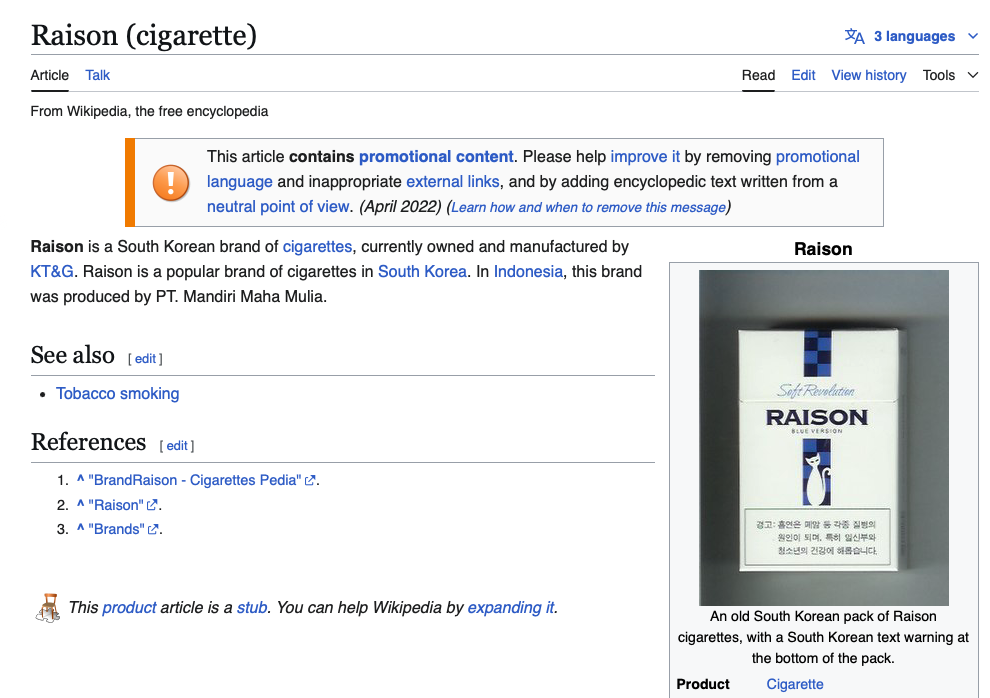
\includegraphics[width=0.6\linewidth]{figures/example_promo_article.png}
        \caption{\url{https://en.wikipedia.org/wiki/Raison\_(cigarette)}}
        \label{fig:enter-label}
    \end{figure}
\end{frame}

\begin{frame}{Problemstellung}
    \begin{block}{Wann ist ein Wikipedia-Artikel gut?}
        \begin{itemize}
            \item redaktionelle Standards (Good article Kriterien)
            \begin{itemize}
                \item gut geschrieben
            
                \item korrekte und \"uberpr\"ufbare Informationen

                \item neutral in der Sichtweise

                \item verwenden Bilder mit geeigneten Urheberrechtslizenzen
            \end{itemize}

            \item Good article nomination (GAN)

            \item nur 0.59\% der Wikipedia-Artikel sind gut (1 von 171)
        \end{itemize}
    \end{block}

    \begin{block}{Problemstellung}
        Ist ein gegebener Wikipedia-Artikeln gut oder promotional? \\

        Zusatz: Falls ein Wikipedia-Artikel nicht gut ist, warum?
    \end{block}
\end{frame}

\section{Daten}

% 54116 gelabelte Wikipedia Artikel
\begin{frame}{Daten}
    \begin{figure}
        \centering
        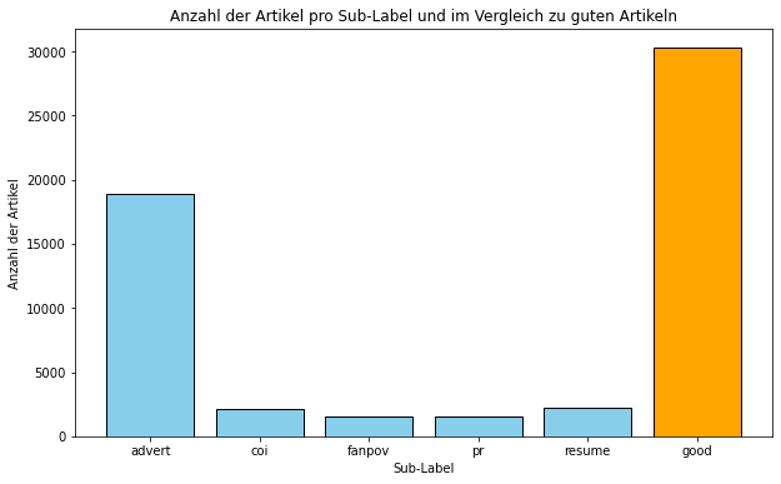
\includegraphics[width=0.8\linewidth]{figures/distribution_multiple_classes.png}
    \end{figure}
\end{frame}

\section{Ans\"atze}

\subsection{Logistische Regression}

\begin{frame}{Logistische Regression (1)}
    \begin{block}{Datenvorverarbeitung}
        \begin{itemize}
            \item Entfernung von Sonderzeichen und Kleinbuchstabierung (nativ durch TF-IDF-Vektorisierung)
            \item Stopw\"orter entfernt, aber Zahlen beibehalten
            \item Optimierung der TF-IDF-Vektorisierung durch Gridsearch:
                  \begin{itemize}
                      \item Maximale Anzahl von Features: \{5000, \textbf{10000}, 20000\}
                      \item n-Gramm-Bereich: \{(1,1), (\textbf{1,2}), \dots ,(3,4)\}
                  \end{itemize}
        \end{itemize}
    \end{block}
\end{frame}

\begin{frame}{Logistische Regression (2)}
    \begin{block}{Methode}
        \begin{itemize}
            \item Klassifikation mit \texttt{LogisticRegression}:
                  \begin{itemize}
                      \item Solver: \texttt{lbfgs}, \texttt{saga}
                      \item Strafterm: \(L1\) oder \(L2\)-Regularisierung
                      \item Multi-Class: \texttt{OneVsRestClassifier} f\"ur multilabel-Klassifikation
                  \end{itemize}
            \item Optimierung des Modells:
                  \begin{itemize}
                      \item Gridsearch f\"ur Hyperparameter der logistischen Regression:
                            \begin{itemize}
                                \item Regularisierungsparameter \(C\): \{0.01, 0.1, 1, 10, 100\}
                                \item Verschiedene Solver (\texttt{lbfgs}, \texttt{saga})
                            \end{itemize}
                      \item \textcolor{red}{Umgang mit Klassenungleichgewicht}: Easy Data Augmentation (EDA) mit nltk.
                            \begin{itemize}
                                \item Synonym Replacement: Es werden zuf\"allig n W\"orter durch Synonyme ersetzt und als neuer Text mit gleichem Label ausgegeben.
                                \item In Pr\"ufung: Random Swap, Random Insertion und Random Deletion
                            \end{itemize}
                  \end{itemize}
        \end{itemize}
    \end{block}
\end{frame}

\begin{frame}{Logistische Regression (3)}
    \begin{block}{Ergebnisse}
        \textcolor{red}{Bild von Ergbenissen}
        %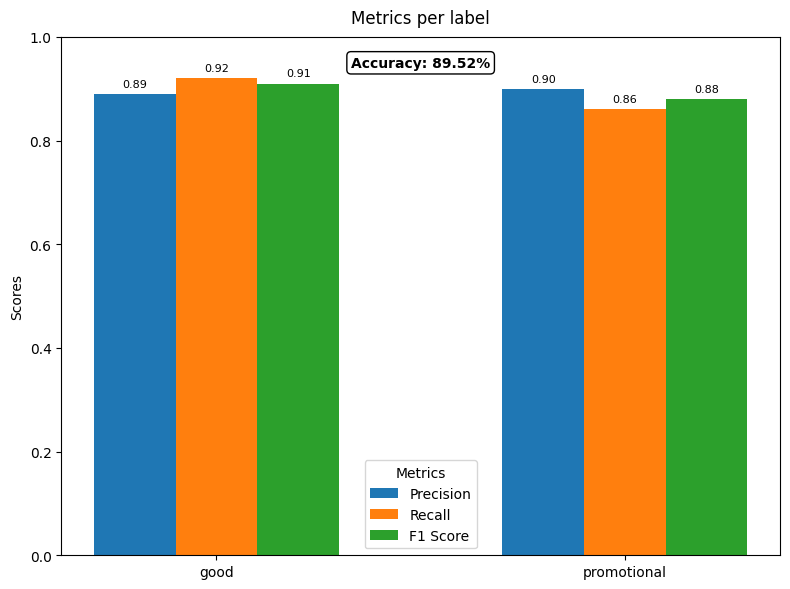
\includegraphics[width=6.8cm]{figures/evaluation_nbb.png} 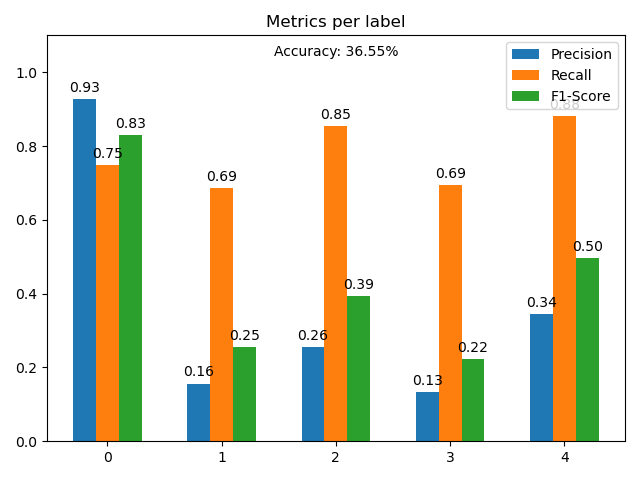
\includegraphics[width=6.8cm]{figures/evaluation_nbm.png}
    \end{block}
\end{frame}

\subsection{Support Vector Machine}

\begin{frame}{Support Vector Machine (1)}
    \begin{block}{Methode}
        \begin{itemize}
            \item TF-IDF-Vektorisierung
            \item Vergleich verschiedener Kernels:
                \begin{itemize}
                    \item \texttt{linear}, \texttt{poly}, \texttt{rbf}, \texttt{sigmoid}.
                    \item Keine Vorteile gegen\"uber \texttt{linear} festzustellen.
                    \item \texttt{LinearSVC} mit deutlich geringerer Laufzeit.
                    \item Parameter-Tuning mit \texttt{GridSearchCV}.
                \end{itemize}
            \item \textbf{Bin\"are Klassifikation}:
                \begin{itemize}
                    \item \texttt{LinearSVC} liefert Precision, Recall, F1-Score und Accuracy jeweils 0.96 - 0.97.
                \end{itemize}
            \item \textbf{Multilabel-Klassifikation}:
                \begin{itemize}
                    \item Klassifikation mit \texttt{MultiOutputClassifier} und \texttt{LinearSVC}.
                    \item Nur \texttt{advert} einigerma\ss{}en identifizierbar mit F1-Score 0.86.
                    \item Bei \texttt{coi}, \texttt{fanpov}, \texttt{pr}, \texttt{resume} F1-Scores von 0.00 bis 0.45.
                    \item Nicht-lineare Kernels liefern \"ahnliche Ergebnisse.
                \end{itemize}
        \end{itemize}
    \end{block}
\end{frame}

\begin{frame}{Support Vector Machine (2)}
    \begin{block}{Ergebnisse}
        \textcolor{red}{Bild von Ergbenissen}
        %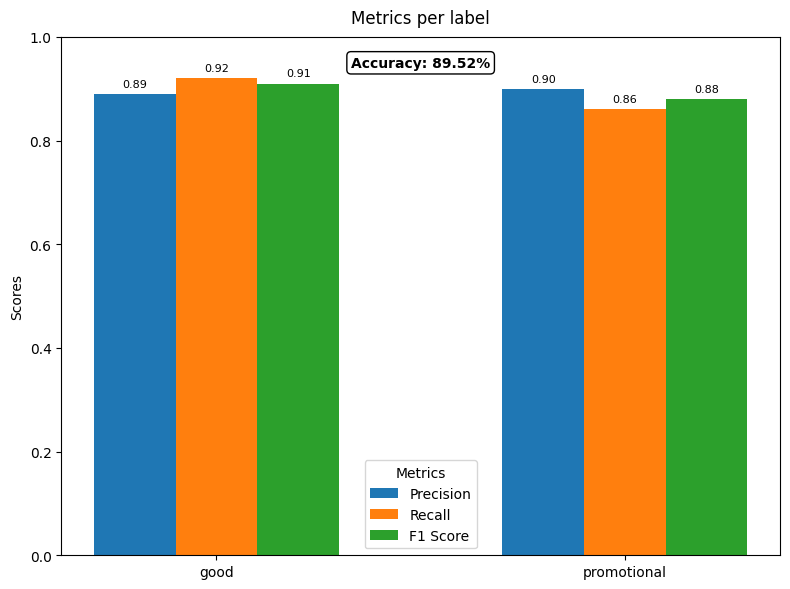
\includegraphics[width=6.8cm]{figures/evaluation_nbb.png} 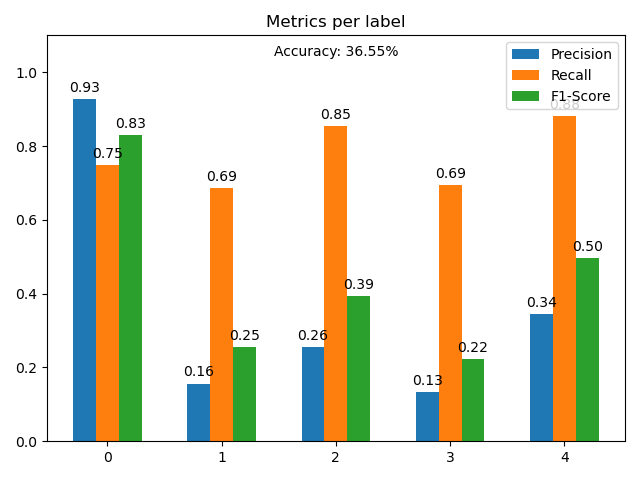
\includegraphics[width=6.8cm]{figures/evaluation_nbm.png}
    \end{block}
\end{frame}

\subsection{Bayes Klassifikator}

\begin{frame}{Bayes Klassifikator (1)}
    \begin{block}{Datenvorverarbeitung}
        \begin{itemize}
            \item Entfernen von Nicht-Wort-Zeichen
            \item Umwandlung in Kleinbuchstaben
            \item Entfernung von f\"uhrenden und folgenden Leerzeichen
            \item Beibehaltung von Stoppw\"ortern und Zahlen (KPIs nicht beeinflusst)
        \end{itemize}
    \end{block}
\end{frame}
\begin{frame}{Bayes Klassifikator (2)}
    \begin{block}{Methode}
        \begin{itemize}
            \item Textrepr\"asentation mittels TF-IDF-Vektorisierung:
                  \begin{itemize}
                      \item Maximale Anzahl von Features: 10.000
                      \item n-Gramm-Bereich: Unigramme (1,1)
                      \item Minimale Dokumentenfrequenz (\texttt{min\_df}): 0.001
                      \item Maximale Dokumentenfrequenz (\texttt{max\_df}): 0.9
                  \end{itemize}
            \item Einstellung des Gl\"attungsparameters \(\alpha = 1.0\)
            \item \textbf{Bin\"are Klassifikation}:
                  \begin{itemize}
                      \item Einsatz von \texttt{MultinomialNB} f\"ur die Klassifikation zwischen promotional und nicht-promotional Artikeln
                  \end{itemize}
            \item \textbf{Multilabel-Klassifikation}:
                  \begin{itemize}
                      \item Verwendung von \texttt{OneVsRestClassifier} mit \texttt{MultinomialNB} f\"ur die Klassifikation in mehrere Klassen
                      \item Behandlung des Klassenungleichgewichts durch Oversampling mit \texttt{RandomOverSampler}
                  \end{itemize}
        \end{itemize}
    \end{block}
\end{frame}

\begin{frame}{Bayes Klassifikator (3)}
    \begin{block}{Ergebnisse}
        \begin{figure}
            \centering
            
            \subfloat {{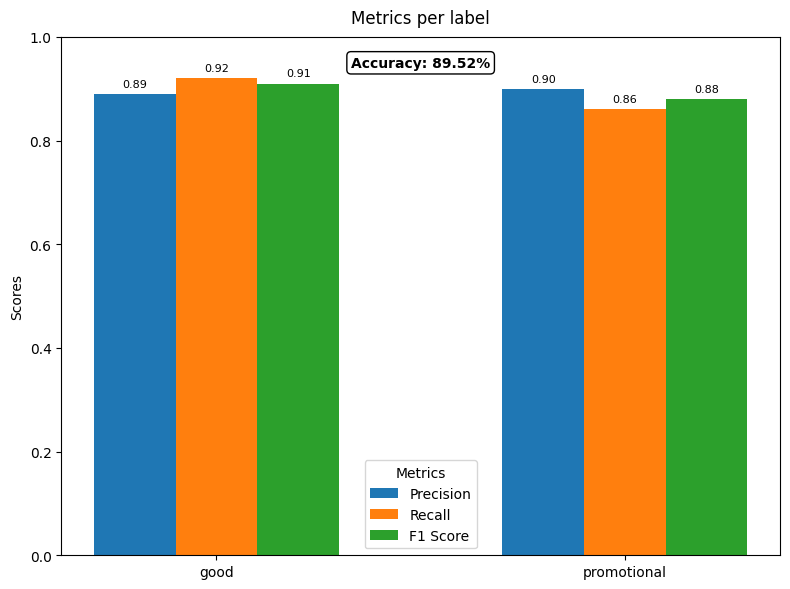
\includegraphics[width=.4\textwidth, height=5cm]{figures/evaluation_nbb.png}}}
            \qquad
            \subfloat {{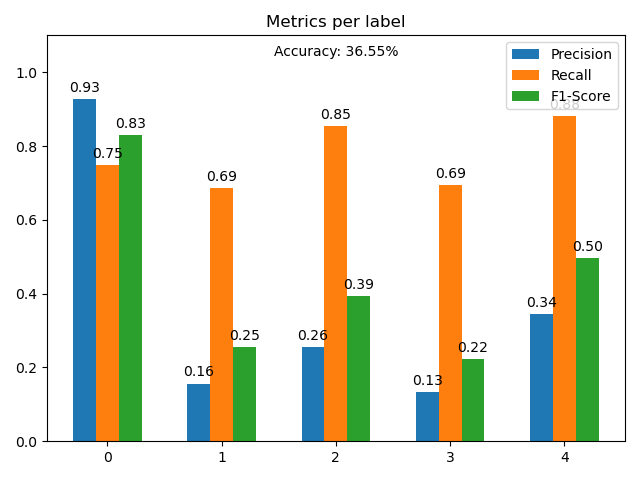
\includegraphics[width=.4\textwidth, height=5cm]{figures/evaluation_nbm.png}}}
        \end{figure}
    \end{block}
\end{frame}

\subsection{Convolutional Neural Network}

\begin{frame}{Convolutional Neural Network (1)}
    \begin{block}{Datenvorverarbeitung}
        \begin{itemize}
            \item Textrepr\"asentation mittels Byte Pair Encoding (\texttt{cl100k\_base})

            \item gegebenenfalls Padtokens erg\"anzen
    
            \item Konvertierung in \texttt{PyTorch Tensor}

            \item als \texttt{PyTorch Dataset} implementiert
        \end{itemize}
    \end{block}

    \begin{block}{Methode}
        \begin{itemize}
            \item Embedding Layer
            \begin{itemize}
                \item ein Embeddingvektor pro Token

                \item auf diesem Layer wird die Faltungsoperation angewendet
            \end{itemize}

            \item \texttt{Conv1d} Layer: Sliding Window um Wikipedia-Artikel zu analysieren

            \item Pooling Layer um Features zusammenzufassen
        \end{itemize}
    \end{block}
\end{frame}

\begin{frame}{Convolutional Neural Network (2)}
    \begin{block}{Training/Optimierung}
        \begin{itemize}
            \item Modellparameter
            \begin{itemize}
                \item Tokenizer

                \item Embedding Dimension

                \item Anzahl Conv Layers

                \item Maximale L\"ange

                \item Dropout

                \item Filtergr\"o{\ss}en

                \item FFN
            \end{itemize}

            \item Trainingsparameter
            \begin{itemize}
                \item Learning Rate

                \item Batch Size

                \item Epochen
            \end{itemize}
            
            \item GridSearch um gute Paramterkonfiguration systematisch zu finden
        \end{itemize}
    \end{block}
\end{frame}

\begin{frame}{Convolutional Neural Network (3)}
    \begin{block}{Ergebnisse}
        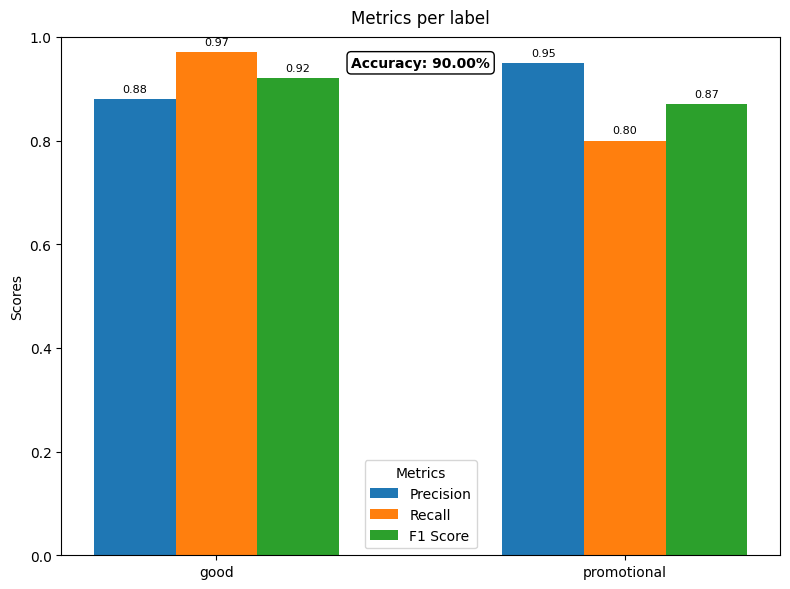
\includegraphics[width=6.8cm]{figures/evaluation_cnnb.png} 
    \end{block}
\end{frame}

\section{Ausblick}
\begin{frame}{Ausblick}
    \begin{block}{Ausblick}
        \begin{itemize}
            \item Hyperparameter-Optimierung
